\chapter{The dictionary learning improvement under smoothness constraints}
\section{The point we started from: \textit{"Learning Parametric Dictionaries for Signals of Graphs"}}
As we previously hinted, in the work of Thanou, Shuman and Frossard the focus was on learning the parametric functions ($kernels$) through which it was possible to reconstruct the graph signal. Moreover, in their work they modelled the graph signal as a combination of overlapping local patterns, describing localized events on the graph which can appear in several vertices. This representation of the graph signal brought to a representation of the dictionary structure that as a concatenation of subdictionaries that are polynomials of the graph Laplacian. Under this assumption, they then learned the coefficients of the kernels through a numerical optimization.

\subsection{The dictionary structure and main assumptions}
To be specific, the dictionary structure we used which is presented in \cite{Thanou2014} is in the following form.: we designed a graph dictionary $\mathcal{D} = [\mathcal{D}_1, \mathcal{D}_2,\dots,\mathcal{D}_S]$, or a concatenation of a set of $S$ subdictionaries, as:
\begin{equation}
  \mathcal{D}_s = \hat{g_s}(\mathcal{L}) = \rchi (\sum_{k=0}^K \alpha_{sk}\Lambda^k)\rchi^T =   \sum_{k=0}^{K} \alpha_{sk}\mathcal{L}^k
\end{equation}
where $\hat{g_s}$ is the pattern (\textit{the kernel}) of the subdictionary $\mathcal{D}_s$ and where the atom given by the $n^{th}$ column of subdictionary $\mathcal{D}_s$ is equal to $\frac{1}{\sqrt{N}}T_ng_s$, the translation operator defined in \autoref{eq:translation} divided by the constant $\frac{1}{\sqrt{N}}$.\\
However, despite the polynomial constraint guarantees the localization of the atoms in the vertex domain, it does not provide though any information about the spectral representation of the atoms. For this reason we included in our problem also the two matrix inequalities already listed in the constraints list of the optimization problem in \ref{eq:overallProblem}:
\begin{align}
  0 \preceq \text{ } &\mathcal{D}_s \preceq cI, \quad \forall s \in \{1,2,\dots , S\},  \label{eqn:boundness}\\
  &\text{and}\\
  (c-\epsilon)I \preceq &\sum_{s=1}^{S}D_s \preceq (c+\epsilon)I \label{eqn:spectrum}
\end{align}
\autoref{eqn:boundness} accounts for the fact that our kernels are nonnegative and uniformly bounded by a given constant $c$ (which we will further suppose equal to 1), while \autoref{eqn:spectrum} accounts for the fact that the signals we consider usually contain frequency components spread across the entire spectrum and so the kernels should cover it as well. These two spectral constraints together contribute to increase the stability of the dictionary.\\

Finally, we underline the fact that for the design of the dictionary the eigenvectors used are the ones from the normalized graph Laplacian, since this configuration revealed to be more suitable for our bodywork.


\section{The dictionary learning algorithm under smoothness constraints}
With these basis we therefore implemented a dictionary learning algorithm based on the one presented in \cite{Thanou2014} in order to add the smoothness priors. As previously mentioned, we can cast the general problem as the following optimization problem:
\begin{align}
  \argmin_{\small{\alpha \in \R^{(K+1)*S}, \text{ } X \in \R^{SN \times N}}} &||Y-DX||^2_F + \mu ||\alpha||_2^2 \label{eq:objDictionary}\\
  \text{subject to} \quad &||x_m||_0 = T_0, \quad \forall m \in \{1,\dots,M\} \notag \\
  &\mathcal{D}_s = \sum_{k=0}^{K}\alpha_{sk}\mathcal{^k}, \quad \forall s \in \{1,2,\dots,S\} \notag \\
  &0 \preceq \text{ } \mathcal{D}_s \preceq cI, \quad \forall s \in \{1,2,\dots , S\},\notag \\
  &(c-\epsilon)I \preceq \sum_{s=1}^{S}D_s \preceq (c+\epsilon)I \notag
\end{align}
with $\mu$ being the coherence coefficient \cri{verifica se è la coherence ciò di cui si parla qui} $x_m$ corresponding to the $m^{th}$ column of the sparsity matrix $X$, $T_0$ being the sparsity level of the coefficient of each signal and the $l_0$ norm term one time more standing for the sparsity need we manifested before.\\

Since the optimization problem is non convex, there is the need to approximate it by the alternation of two optimization convex subproblems, namely the sparse coding and the dictionary update step.\\

The sparse coding step aims at learning the sparsity matrix $X$ solving
\begin{equation}
  \argmin_{X} ||Y - DX||^2_F \qquad \text{subject to} \quad ||x_m||_0 \leq T_0,
\end{equation}
and it is solved using the \gls{omp} method, an iterative greedy algorithm that at each step selects the element in the dictionary that is best correlated with the signal residual part; it subsequently produces a new estimation through the projection of the signal onto the dictionary elements that have already been selected. This method admits simple and fast implementation and it has been proved that his error on the approximation is only a small factor worse than the minimal error obtained through a non-sparse representation. \cite{Tropp2004}.\\

On the other side, the dictionary update step aims at finding the polynomial coefficients of the kernels by minimizing
\begin{equation}
  \argmin_{\alpha \in \R^{(K+1)S}} ||Y - DX||^2_F + \mu||\alpha||_2^2
\end{equation}
subject to the remaining constraints in \autoref{eq:objDictionary}
\cri{in caso più avanti aggiungi la parte su $P_{nm}^s$ se vedi che si rivela utile}

To this main problem we then added the smoothness prior through two different implementations, the first one trying to insert the smoothness assumption inside the objective function of the dictionary update step, while the second one focusing on adding a smoothness prior in the constraints of the optimization function.

\subsection{Smoothness prior in the objective function}
We remember the equations \ref{eq:polynom}, and we reformulate them as
\begin{equation}
  g(\lambda) = \sum_{k=0}^K\alpha_k \lambda^k = \sum_{n=0}^N\gamma_n \lambda^n \times \sum_{m=0}^M  \beta_m \lambda^m
  \label{eq:giLambda}
\end{equation}
With $h(\lambda) = \sum_{n=n}^N \gamma_n \lambda^n$ and $(\lambda - \lambda_M)(\lambda - \lambda_{M-1})\cdot_{\dots}\cdot (\lambda - \lambda_{M - N +1})$ being the two subpolynomials in which \ref{eq:giLambda} has been decomposed. B Between these, $h(\lambda)$ represents the polynomial with the unknown coefficients to be found, while the polynomial in the unknown $\beta$ is the one obtained from imposing the highest eigenvalues as roots of the general polynomial \ref{eq:giLambda} \cri{torna nelle sezioni indietro per sistemare gli indici del polinomio h} Since we deal with the optimization problem in \autoref{eq:objDictionary} through linear matrix inequality tools, we try to model the vector containing the kernel coefficients in such a way that its structure itself already holds the information regarding the structure of the two sub polynomials. To do so, we multiply the two sub polynomials among each other without resolving the equation with known $\beta$, but leaving them as unknown, in such a way that the behavior of the overall polynomial emerges. We thus obtain the structure that every $\alpha$ coefficient should have in order to transmit the smoothness prior to the objective function. Namely:
\begin{equation}
  \begin{split}
    \sum_{n=0}^N\gamma_n \lambda^n \times \sum_{m=0}^M \beta_m \lambda^m &= (\beta_0  \gamma_0)\lambda^0   + (\beta_0 \gamma_1 + \beta_1 \gamma_0)\lambda + \dots + \\
    &(\beta_0 \gamma_N + \beta_1 \gamma_{N-1} + \dots + \beta_N \gamma_0)\lambda^N + \dots + \\
    &(\beta_1 \gamma_N + \beta_2 \gamma_{N-1} + \dots + \beta_{N+1} \gamma_0)\lambda^{N+1} + \dots +\\
    &(\beta_{N} \gamma_{N} + \beta_{N+1} \gamma_{N-1} + \dots + \beta_{M} \gamma_0)\lambda^{M} + \\
    &(\beta_{N+1} \gamma_{N} + \dots + \beta_{2N + 1} \gamma_1)\lambda_{M+1} + \dots +\\
    &(\beta_M \gamma_N)\lambda^{K}
  \end{split}
  \label{eq:sviluppo}
\end{equation}
Once we obtained it, we insert this knew knowledge over the kernels structure in the optimization objective function, where now the alpha vector has a reduced number of unknowns that have to be found. With the problem set in this way we can then analyse the new results we obtain. \cri{verifica se nei punti precendenti hai dato abbastanza spazio a questo concetto di smoothness e di come si comporta un grapho soggetto a questa struttura, se non è così ribidisci il fatto che ci interessa sapere altro sulla smth perchè così il grafo risulta più frammentato e in passi successivi separarlo ptrebbe essere un notevole vantaggio}

\subsection{Smoothness prior in the optimization constraints}
\cri{qui spiega meglio la motivazione quando avrai una funzione decente per l'altra soluzione}
Another approach to the problem is to insert this smoothness prior in the constraints of the optimization function, on one side this choice should be discarded in favour of the first approach, since adding other constraints to our already ill posed problem could add more non-desired complexity; on another side this choice could reveal motivated by the fact that the control over the behavior of the optimization algorithm is in this way more verifiable than in the previous case, in which a black-box-stile coefficients vector detains all the smoothness priors. In this case the constraint added is the imposition that the Vandermonde matrix, obtained selecting only the last $M$ high-frequency eigenvalues in the graph Laplacian, should of course give a null vector when multiplied by the vector of the alpha coefficients. If $P$ is the total number of nodes in the considered graph, then we have:
\begin{equation}
  \begin{bmatrix}
    1 & \lambda_{P-M} & \lambda_{P-M}^2 & \dots & \lambda_{P-M}^{K} \\
    1 & \lambda_{P-M+1} & \lambda_{P-M+1}^2 & \dots & \lambda_{P-M+1}^{K} \\
    \vdots & & \\
    1 & \lambda_P & \lambda_P^2 & \dots & \lambda_P^K \\
\end{bmatrix}
\begin{bmatrix}
  \alpha_0 \\
  \alpha_1 \\
  \vdots \\
  \alpha_K
\end{bmatrix}
=
\begin{bmatrix}
  0\\
  0\\
  \vdots\\
  0
\end{bmatrix}
\end{equation}

\subsection{The optimization algorithm}
The final optimization algorithm is in this way described:
\cri{sistema la faccenda della caption in questo algoritmo}
\begin{algorithm}[H]
  % \caption{{Parametric dictionary learning on graph with smoothness priors}
  \begin{algorithmic}[1]
    \Procedure{initialization}{}
      \State $Y \gets \text{Signal samples set}$
      \State $T_0\gets \text{Target sparsity}$
      \State $K \gets \text{Polynomial degree}$
      \State $S \gets \text{Number of subdictionaries}$
      \State $iterNum \gets \text{Number of iterations}$
      \State $\mathcal{D} \gets \text{Initial dictionary computed thirugh random kernels}$
    \EndProcedure
    \For{$i=1,2,\dots, iter$}
      \Procedure{Sparsity step}{}
        \State \text{Scale each atom in $\mathcal{D}$ to a unit norm}
        \State $X \gets \text{Sparsity estimation with \gls{omp}}$
        \State{Rescale $X$ and $\mathcal{D}$ to recover the polynomial structure}
      \EndProcedure
      \Procedure{Dictionary learning step}{}
        $\alpha \gets \text{kernels estimation through sdpt3}$
      \EndProcedure
      \Procedure{Dictionary update step}{}
        \State $\mathcal{D} \gets \sum_{k=0}^K \alpha_k \mathcal{L}^k$
      \EndProcedure
    \EndFor
  \end{algorithmic}
\end{algorithm}

\subsection{Results}
\label{sec:dataGen}
\subsubsection{Data Generation}
The datasets used in the experiments are composed by a signal $Y$, an adjacency matrix $W$ and the comparison kernels used after the algorithm execution to verify the quality of the results. The signal $Y$ is obtained as the repetition of $2000$ samples randomly generated by a uniform distribution, the graph manifold onto which the signal is structured has $30$ nodes (for simplicity reasons) while the edges that are elements of the weight matrix $W$ are generated from the gaussian function
\begin{equation}
  w_{ij} = e^{-\frac{||x_i - x_j||_2^2}{2\sigma^2}}
\end{equation}
following the approach in \cite{Kalofolias2016}. At the same time, the kernel coefficients we generated as ground truth values come respectively:
\begin{itemize}
  \item form the Taylor expansion for the heat kernels
\end{itemize}
\begin{equation}
  \hat{g(\lambda)} \approx e^{-2\lambda}
\end{equation}
\begin{itemize}
  \item and from one of the synthetic kernels used in the dataset from \cite{Thanou2014}
\end{itemize}

\cri{ufficializza i parametri in seguito}
The number of iterations we apply in this first part of the work is $60$, as we found it is a good value for the algorithm to properly converge to a minimum, while the value of $\epsilon$ for the spectral boundaries in \ref{sec:DictionaryLearningSection} has been set to $0.2$. Moreover, we assume the sparsity coefficient $T_0$ to be equal to $4$ and the coherence parameter $\mu$ to $10^{-4}$.

We use the \textit{sdpt3} solver in the \textit{yalmip} optimization toolbox to solve the quadratic problem and, in order to directly compare the methods here described, we always use the \gls{omp} optimization criteria for the sparse coding step.

Finally, the average normalized approximation error we examine for the results quality is defined as \cri{riscrivi la formula a parole tue}
\begin{equation}
  \frac{1}{|Y_{test}|}\sum_{m=1}^{|Y_{test}|}||Y_m - \mathcal{D}X_m||_2^2
\end{equation}
with $|Y_{test}|$ being the cardinality of the testing set.

\subsubsection{First approach: smoothness in the structure}

\subsubsection{Second approach: smoothness in the constraints}
Results show a general improvement, both regarding the reproduction error and the behavior of the kernel coefficients. The experiments have been repeated several times, in order to be able to claim the stability of the algorithm and show a stable trend. The first important value that testify the improvement of the procedure is the reproduction error, since it decreases significantly when the smoothness prior is included in the optimization process. In \autoref{tab:errorHeat} and \autoref{tab:errorDorina} there is a comparison between the error obtained with and without the smoothness assumption, both for the case in which we have one heat kernel and the case in which we used the smooth kernel from the work of Thanou et al.: it can be noticed that its value tends to be stable during several iterations.

\begin{table}[htbp]
  \centering
  \begin{tabular}{c|c|c}
    \multicolumn{1}{c|}{\textbf{Iteration number}} &
    \multicolumn{1}{c}{\textbf{Original algorithm}} &
    \multicolumn{1}{|c}{\textbf{Smoothness assumption}}\\
    \hline
    1 & 0 & 0\\
    2 & 0 & 0\\
    3 & 0 & 0\\
    4 & 0 & 0\\
    5 & 0 & 0\\
  \end{tabular}
  \caption{Reproduction error comparison for the Heat kernel dataset}
  \label{tab:errorHeat}
\end{table}

\begin{table}[htbp]
  \centering
  \begin{tabular}{c|c|c}
    \multicolumn{1}{c|}{\textbf{Iteration number}} &
    \multicolumn{1}{c}{\textbf{Original algorithm}} &
    \multicolumn{1}{|c}{\textbf{Smoothness assumption}}\\
    \hline
    1 & 0 & 0\\
    2 & 0 & 0\\
    3 & 0 & 0\\
    4 & 0 & 0\\
    5 & 0 & 0\\
  \end{tabular}
  \caption{Reproduction error comparison for the low frequency kernel from Thanou et al. dataset}
  \label{tab:errorDorina}
\end{table}

The improvement can then be noticed in the behavior of the kernels' coefficients: in \autoref{fig:alphaHeatDictionary} there is a comparison between the values assumed by the original heat kernels' coefficients (blue lines), and the ones assumed by the learned coefficients in the case we are applying the smoothness prior or not. It can be seen how the coefficients in the case of no smoothness priors tend to have a less defined trend, while in the smoothness case, they follow the original trend more faithfully. This aspect is shown even more clearly in the case of Thanou et al.'s dataset (\autoref{fig:alphaDorinaDictionary}), in which the coefficients have almost the same behavior, apart from their absolute value.

\begin{figure}
  \centering
  \begin{minipage}[c]{.8\textwidth}
    \centering
    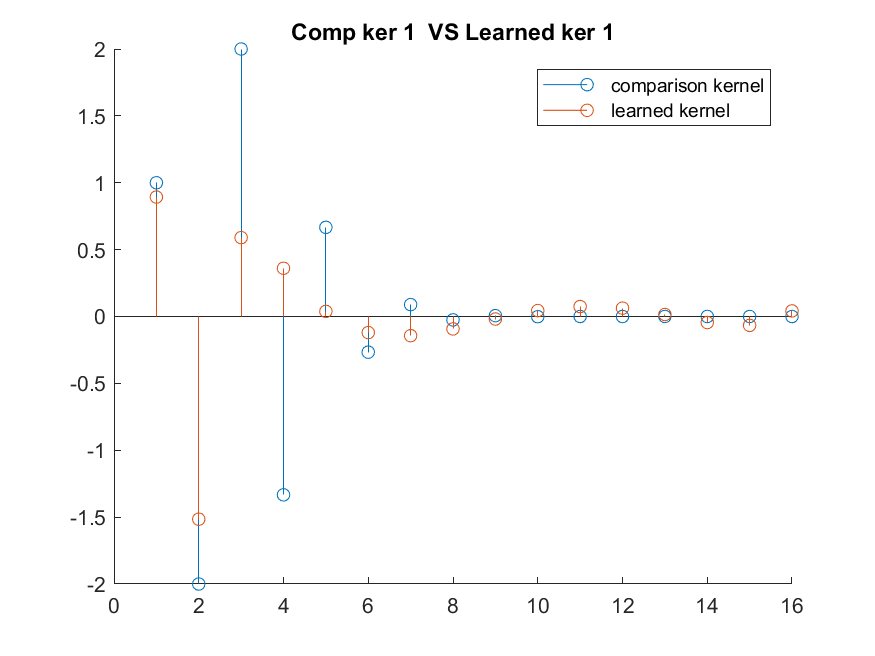
\includegraphics[width = \textwidth]{alphaHeat_noSmoothness_dictionary.png}
  \end{minipage}
  \begin{minipage}[c]{.8\textwidth}
    \centering
    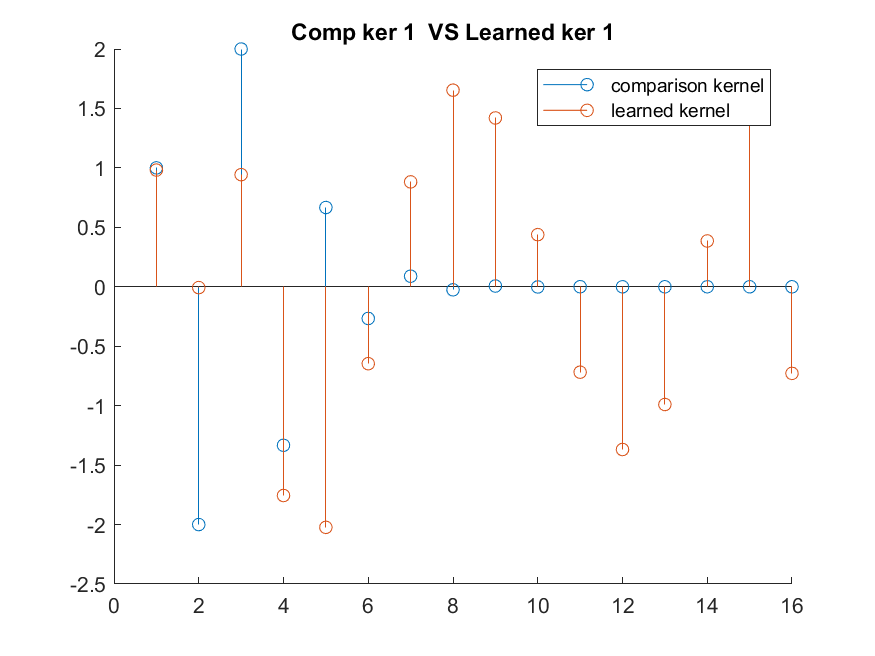
\includegraphics[width = \textwidth]{alphaHeat_Smoothness_dictionary.png}
  \end{minipage}
  \caption{Comparison between kernels coefficients without and with smoothness prior. Heat kernel   dataset}
  \label{fig:alphaHeatDictionary}
\end{figure}

\begin{figure}
  \centering
  \begin{minipage}[c]{.8\textwidth}
    \centering
    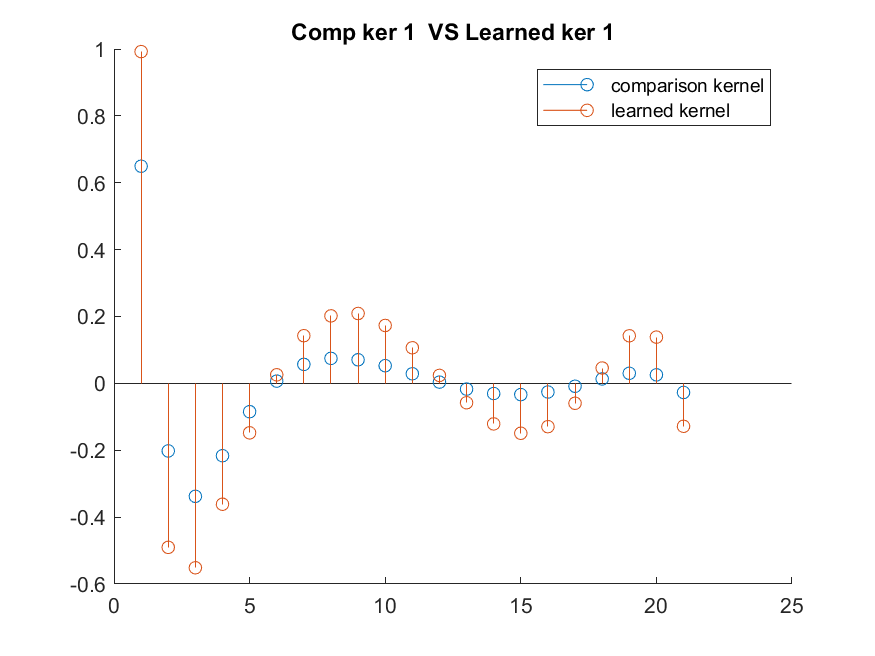
\includegraphics[width = \textwidth]{alphaDorina_noSmoothness_dictionary.png}
  \end{minipage}
  \begin{minipage}[c]{.8\textwidth}
    \centering
    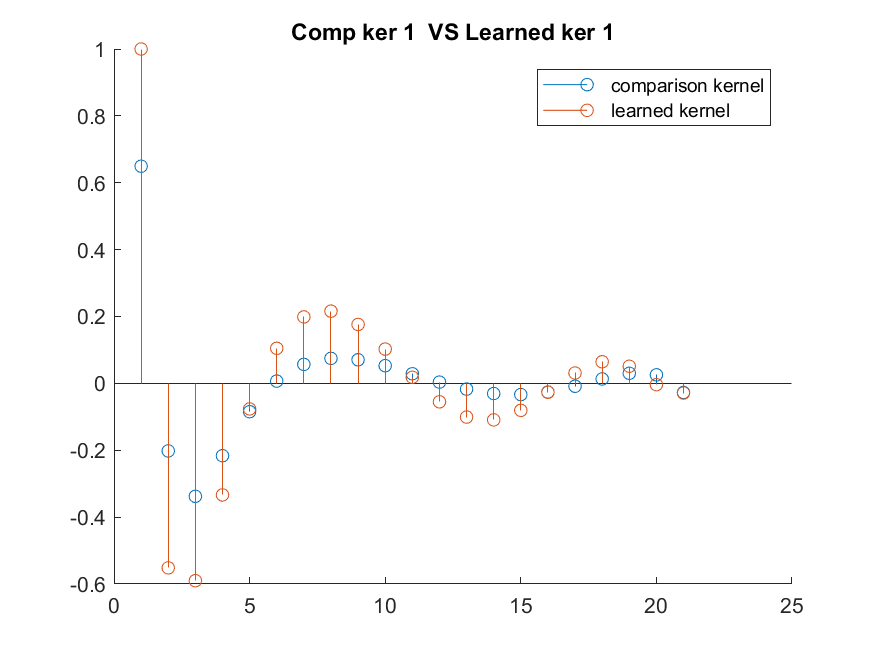
\includegraphics[width = \textwidth]{alphaDorina_Smoothness_dictionary.png}
  \end{minipage}
  \caption{Comparison between kernels coefficients without and with smoothness prior. Thanou et al.   dataset}
  \label{fig:alphaDorinaDictionary}
\end{figure}


Moreover, \autoref{fig:kernelHeatDictionary} and \autoref{fig:kernelDorinaDictionary} show the comparison between the original kernel and the learned kernel without and with smoothness prior in the case of a Heat kernel (\ref{fig:kernelHeatDictionary}) and the dataset from  Thanou et al. (\ref{fig:kernelDorinaDictionary}). It can be seen how the use of smoothness improves the overall trend also for the kernel shape, which is the ultimate purpose of the algorithm.

\begin{figure}
  \begin{minipage}[c]{.5\textwidth}
    \centering
    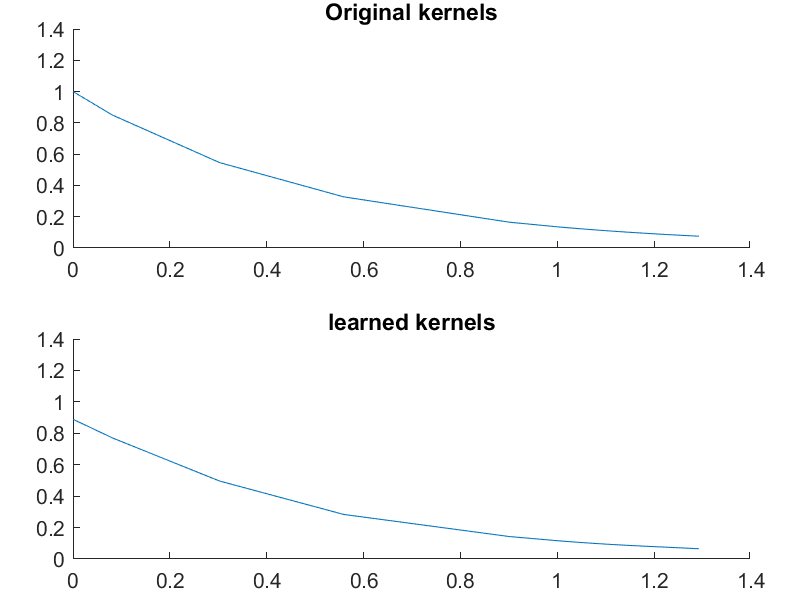
\includegraphics[width = \textwidth]{kernelHeat_noSmoothness_dictionary.png}
  \end{minipage}
  \begin{minipage}[c]{.5\textwidth}
    \centering
    \includegraphics[width = \textwidth]{kernelHeat_Smoothness_dictionary.png}
  \end{minipage}
  \caption{Comparison between kernels without and with smoothness prior. Heat kernel dataset}
  \label{fig:kernelHeatDictionary}
\end{figure}

\begin{figure}
  \begin{minipage}[c]{.5\textwidth}
    \centering
    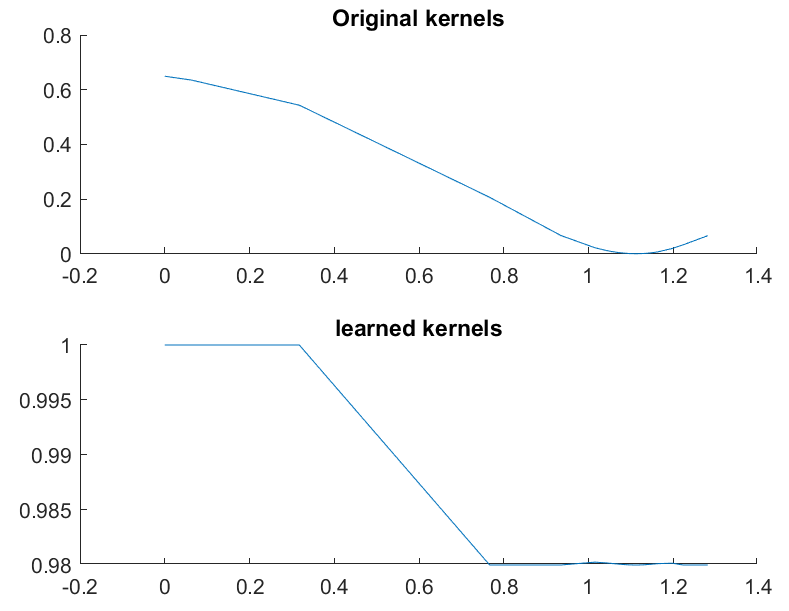
\includegraphics[width = \textwidth]{kernelDorina_noSmoothness_dictionary.png}
  \end{minipage}
  \begin{minipage}[c]{.5\textwidth}
    \centering
    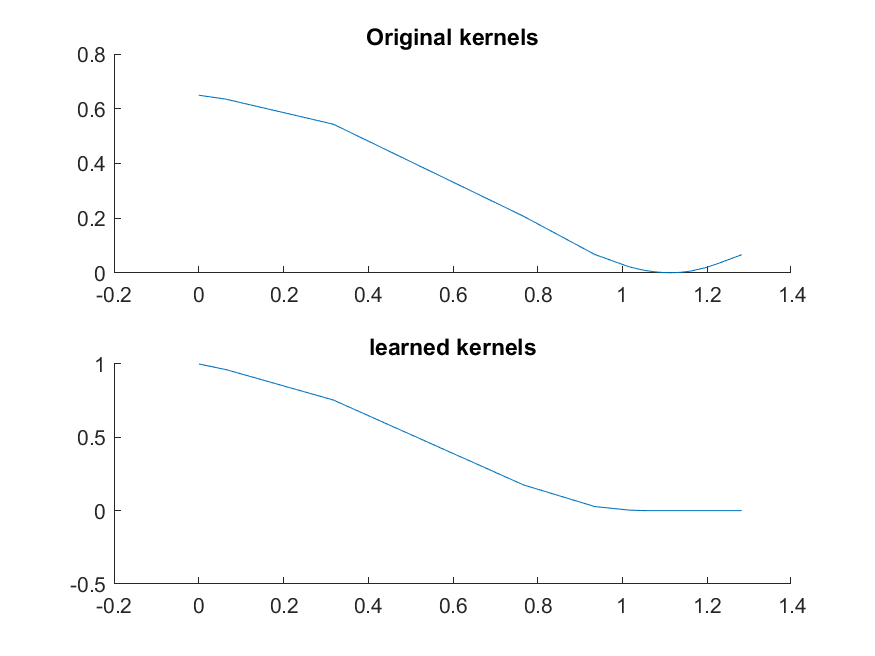
\includegraphics[width = \textwidth]{kernelDorina_smoothness_dictionary.png}
  \end{minipage}
  \caption{Comparison between kernels without and with smoothness prior. Thanou et al. kernel dataset}
  \label{fig:kernelDorinaDictionary}
\end{figure}

Finally, if we look at the behavior of the CPU time necessary for every optimization step, we see that the values in the case we add our prior are in the same order of the ones obtained without it, which gives us further confirmation that out method, despite adding complexity due to the constraints, it does not, though, increase the computational cost.

\begin{figure}
  \begin{minipage}[c]{.5\textwidth}
    \centering
    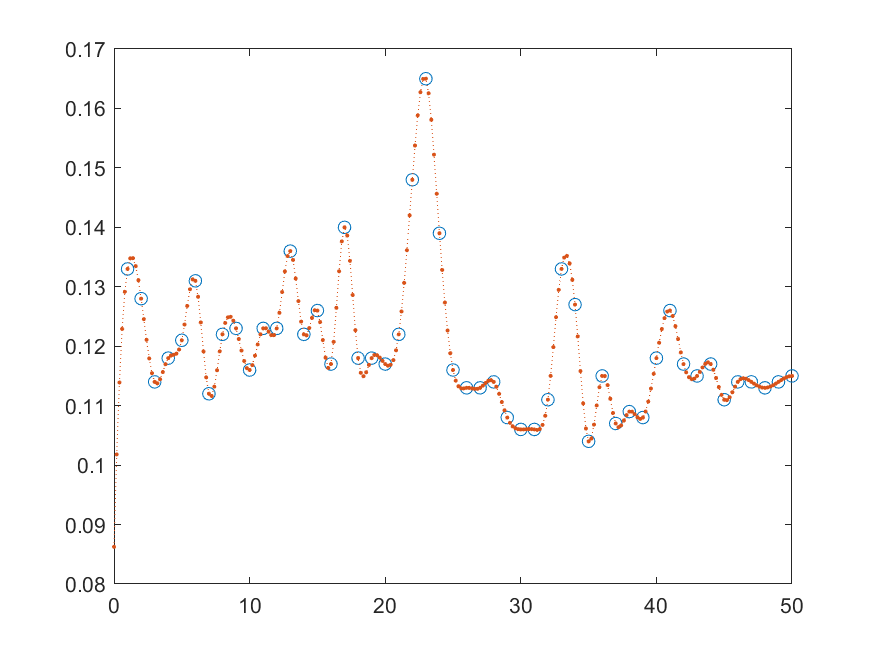
\includegraphics[width = \textwidth]{CPUHeat_noSmoothness_dictionary.png}
  \end{minipage}
  \begin{minipage}[c]{.5\textwidth}
    \centering
    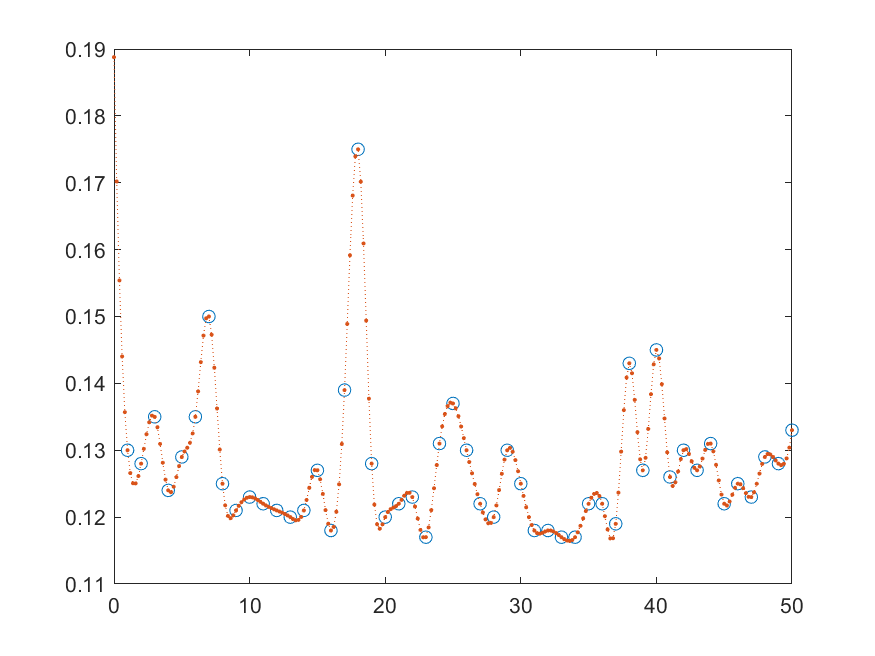
\includegraphics[width = \textwidth]{CPUHeat_Smoothness_dictionary.png}
  \end{minipage}
  \caption{Comparison between kernels without and with smoothness prior. Heat kernel dataset}
  \label{fig:CPUHeatDictionary}
\end{figure}

\begin{figure}
  \begin{minipage}[c]{.5\textwidth}
    \centering
    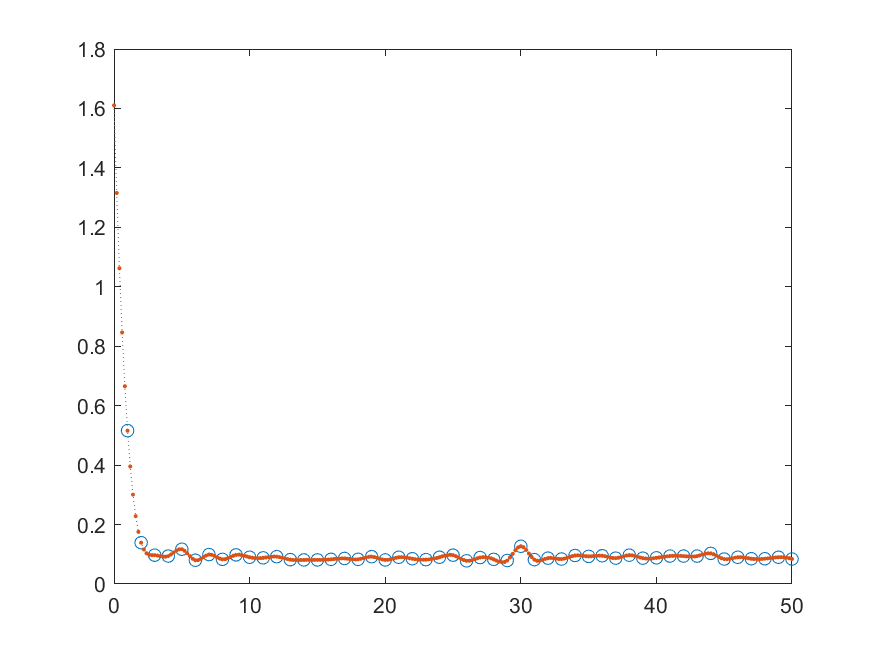
\includegraphics[width = \textwidth]{CPUDorina_noSmoothness_dictionary.png}
  \end{minipage}
    \begin{minipage}[c]{.5\textwidth}
    \centering
  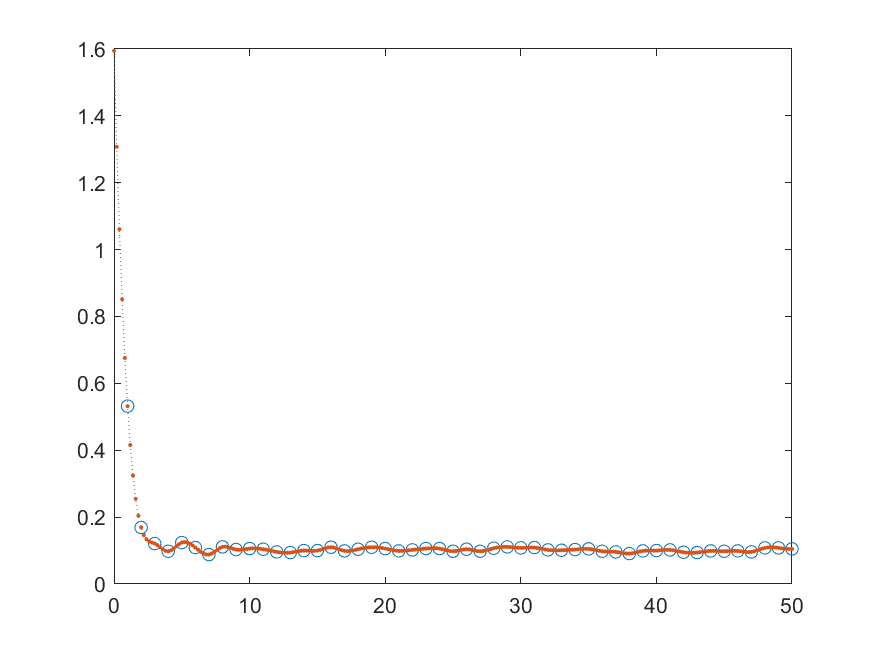
\includegraphics[width = \textwidth]{CPUDorina_Smoothness_dictionary.png}
  \end{minipage}
  \caption{Comparison between kernels without and with smoothness prior. Thanou et al. kernel dataset}
  \label{fig:CPUDorinaDictionary}
\end{figure}
